\documentclass{article}
\usepackage{graphicx} % Required for inserting images

\title{graphs}
\author{Bartek Smolibowski}
\date{March 2024}

\begin{document}

\maketitle

\clearpage
\section{H1}

\textbf{Sprawdzenie hipotezy:  Zwiekszajac n mozna oscylowac blisko liczbie 2Π.}

\begin{figure}[htbp]
    \centering
    
\includegraphics[width=1\textwidth]{~/AlgoNumeryczne/Zadanie1/Grafy/obwod_plot.png}
    \caption{Wykres obwodu.}
    \label{fig:h1}
\end{figure}

\clearpage
\section{H2}

\textbf{Sprawdzenie hipotezy:  Suma wszystkich wektorów wi daje dokaadnie wektor zerowy.}

\begin{figure}[t]
    \centering
    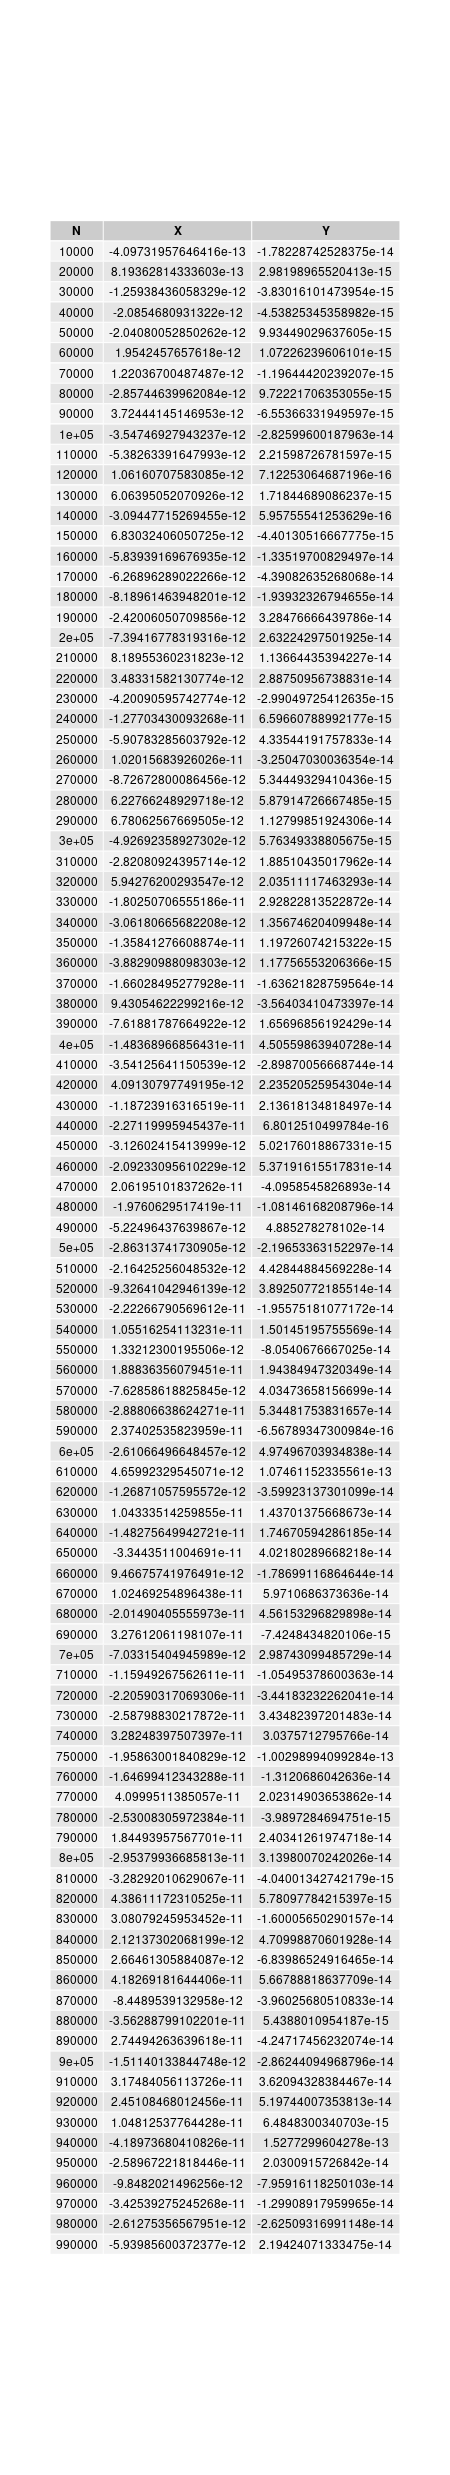
\includegraphics[width=0.5\textwidth]{~/AlgoNumeryczne/Zadanie1/Grafy/h2_table.png}
    \caption{Tabela roznicy.}
    \label{fig:h2}
\end{figure}

\begin{figure}[t]
    \centering
    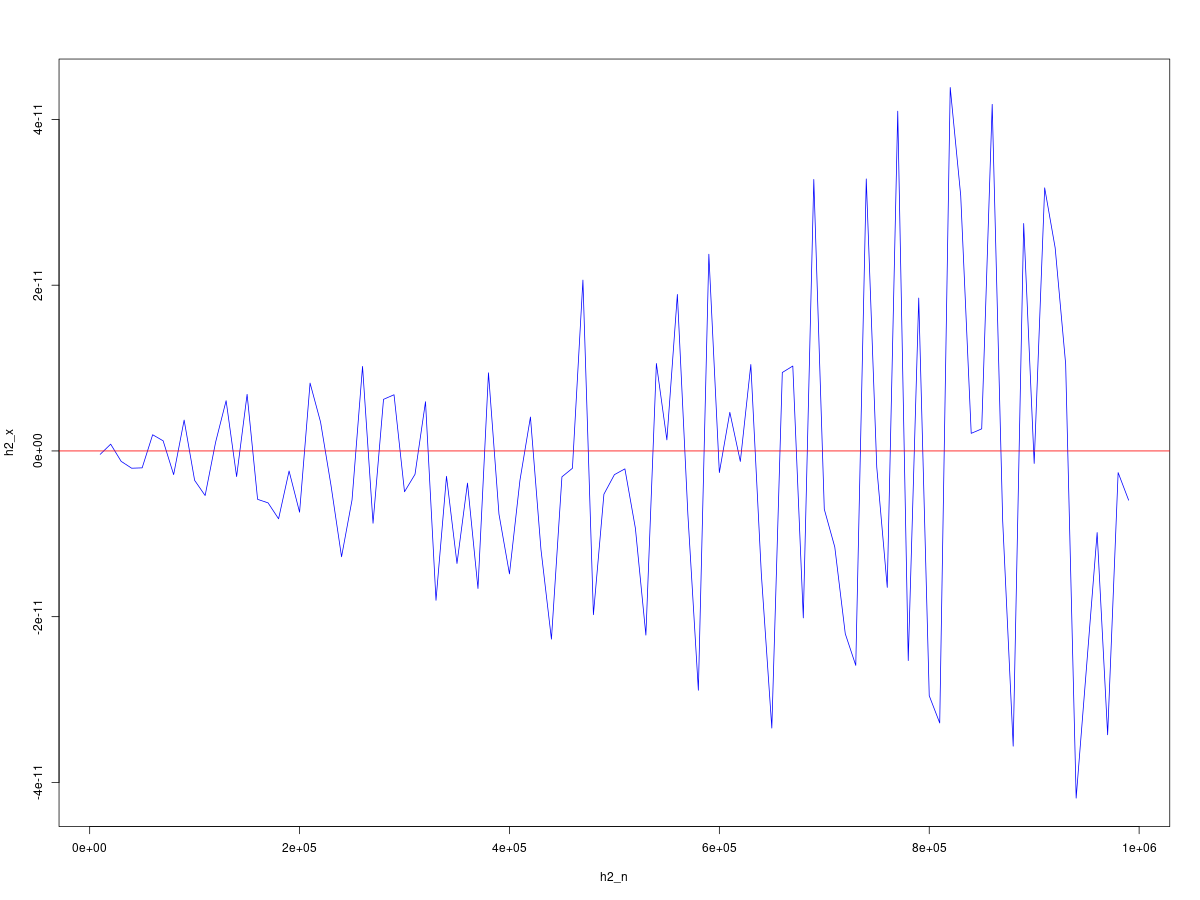
\includegraphics[width=1\textwidth]{~/AlgoNumeryczne/Zadanie1/Grafy/h2X_plot.png}
    \caption{h2 X}
    \label{fig:h2}
\end{figure}

\begin{figure}[t]
    \centering
    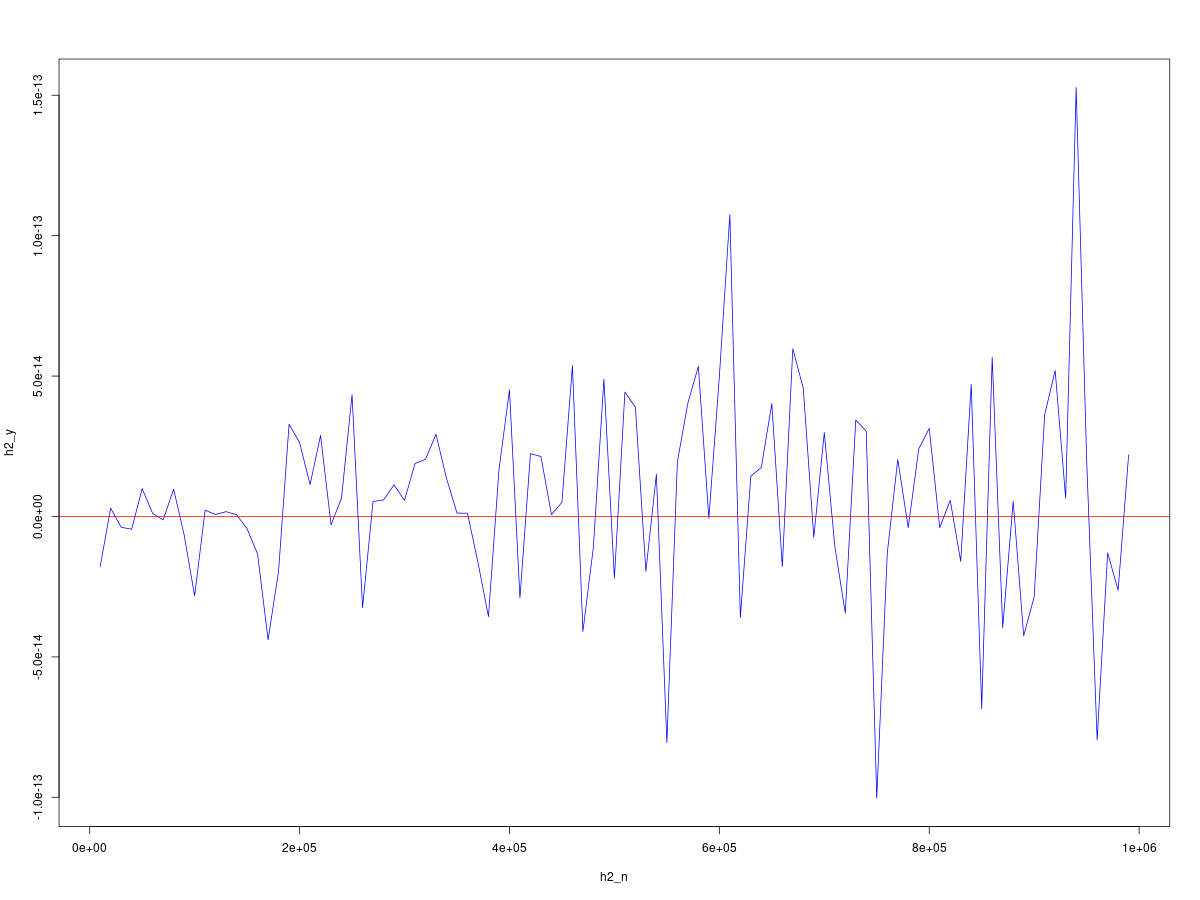
\includegraphics[width=1\textwidth]{~/AlgoNumeryczne/Zadanie1/Grafy/h2Y_plot.png}
    \caption{h2 Y}
    \label{fig:h2}
\end{figure}


\clearpage
\section{H3}

\textbf{Sprawdzenie hipotezy: Gdzie sume wszystkich wspolrzednych wektorow wi mozna policzyc osobno }

\begin{figure}[htbp]
    \centering
    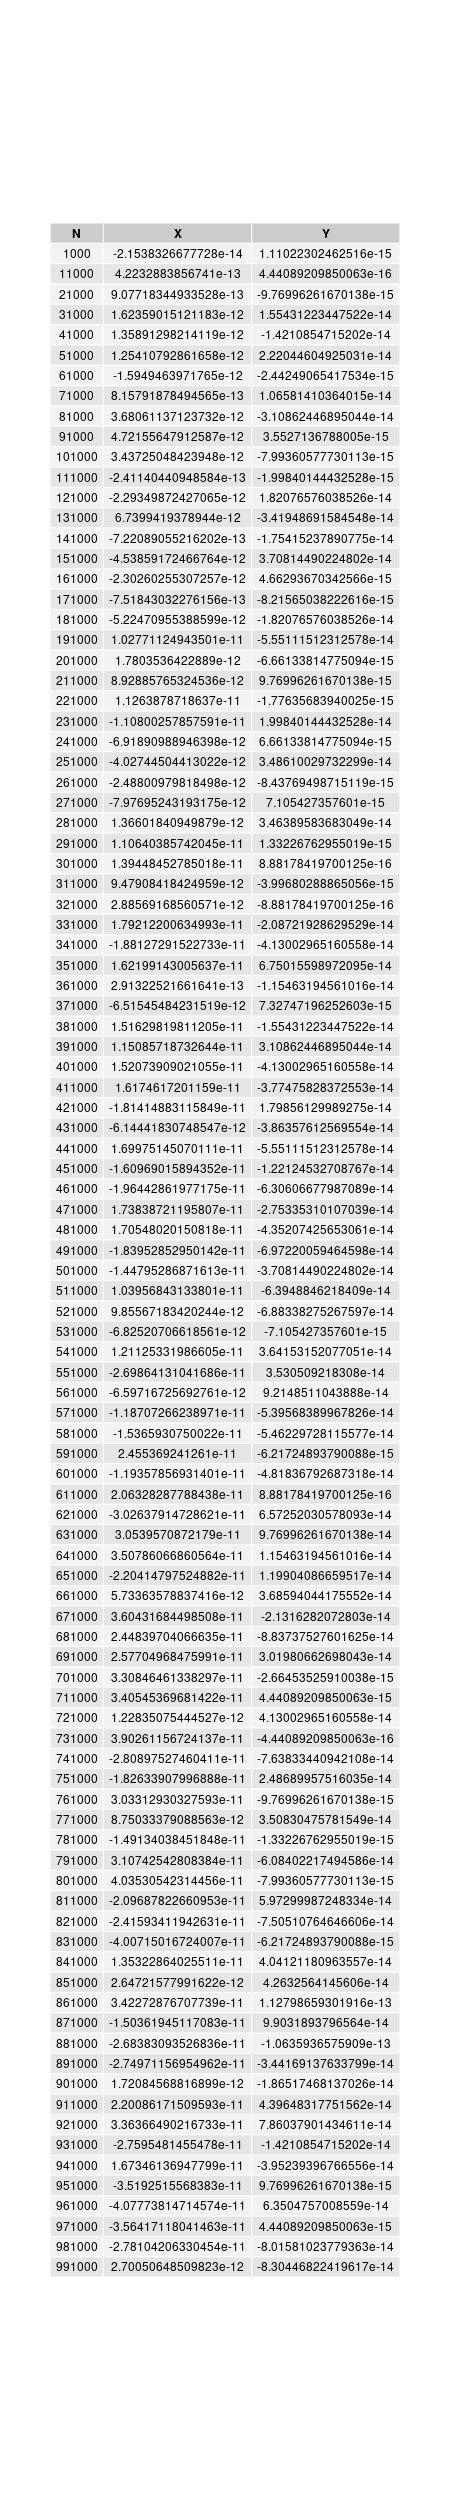
\includegraphics[width=0.5\textwidth]{~/AlgoNumeryczne/Zadanie1/Grafy/h3_table.png}
    \caption{Tabela roznicy h3.}
    \label{fig:h3}
\end{figure}


\begin{figure}[t]
    \centering
    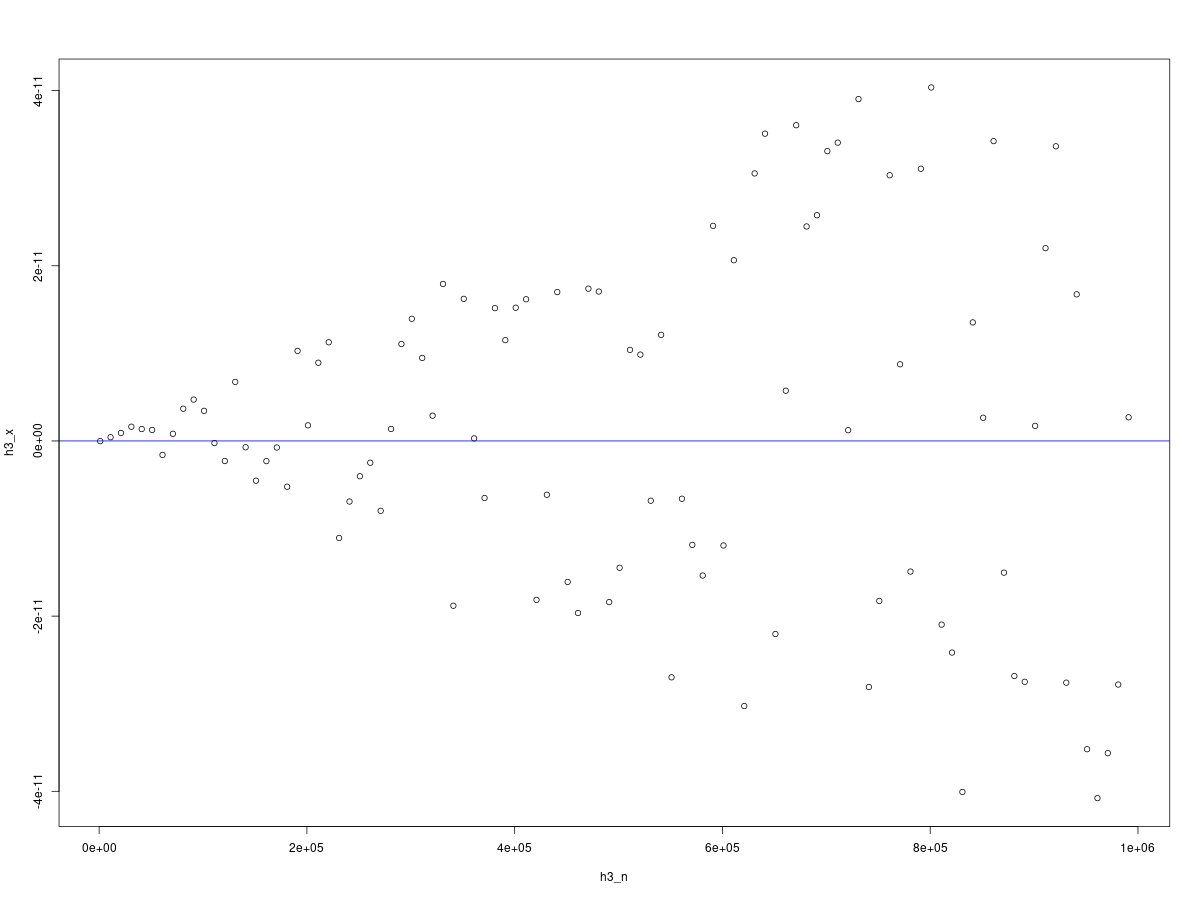
\includegraphics[width=1\textwidth]{~/AlgoNumeryczne/Zadanie1/Grafy/h3X_plot.png}
    \caption{H3x plot .}
    \label{fig:h2}
\end{figure}

\begin{figure}[t]
    \centering
    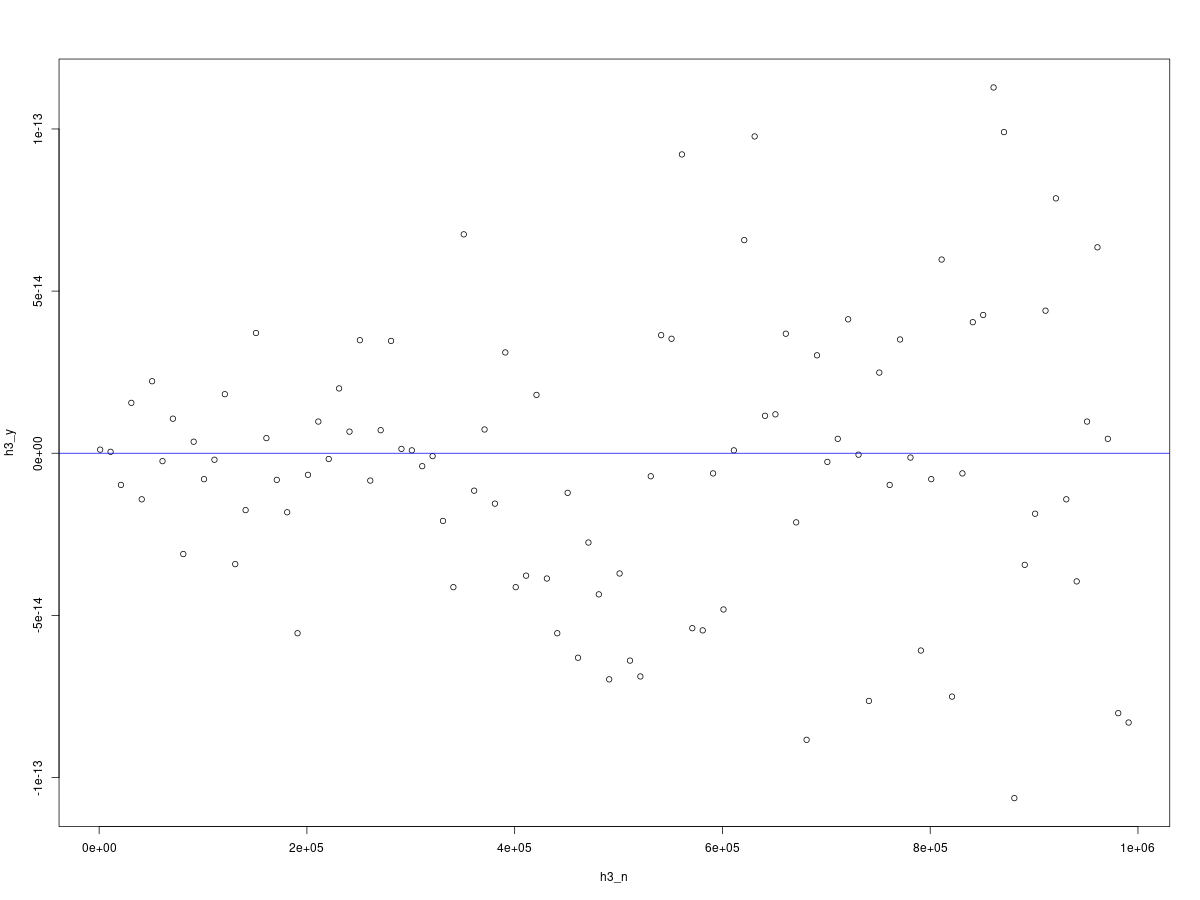
\includegraphics[width=1\textwidth]{~/AlgoNumeryczne/Zadanie1/Grafy/h3Y_plot.png}
    \caption{H3 y plot .}
    \label{fig:h2}
\end{figure}

\clearpage
\section{H4}

\textbf{Sprawdzenie hipotezy: Opisane zastosowanie metody Monte Carlo jest mniej efektywne niz metoda oparta
o sumowanie wektorów }

\begin{figure}[htbp]
    \centering
    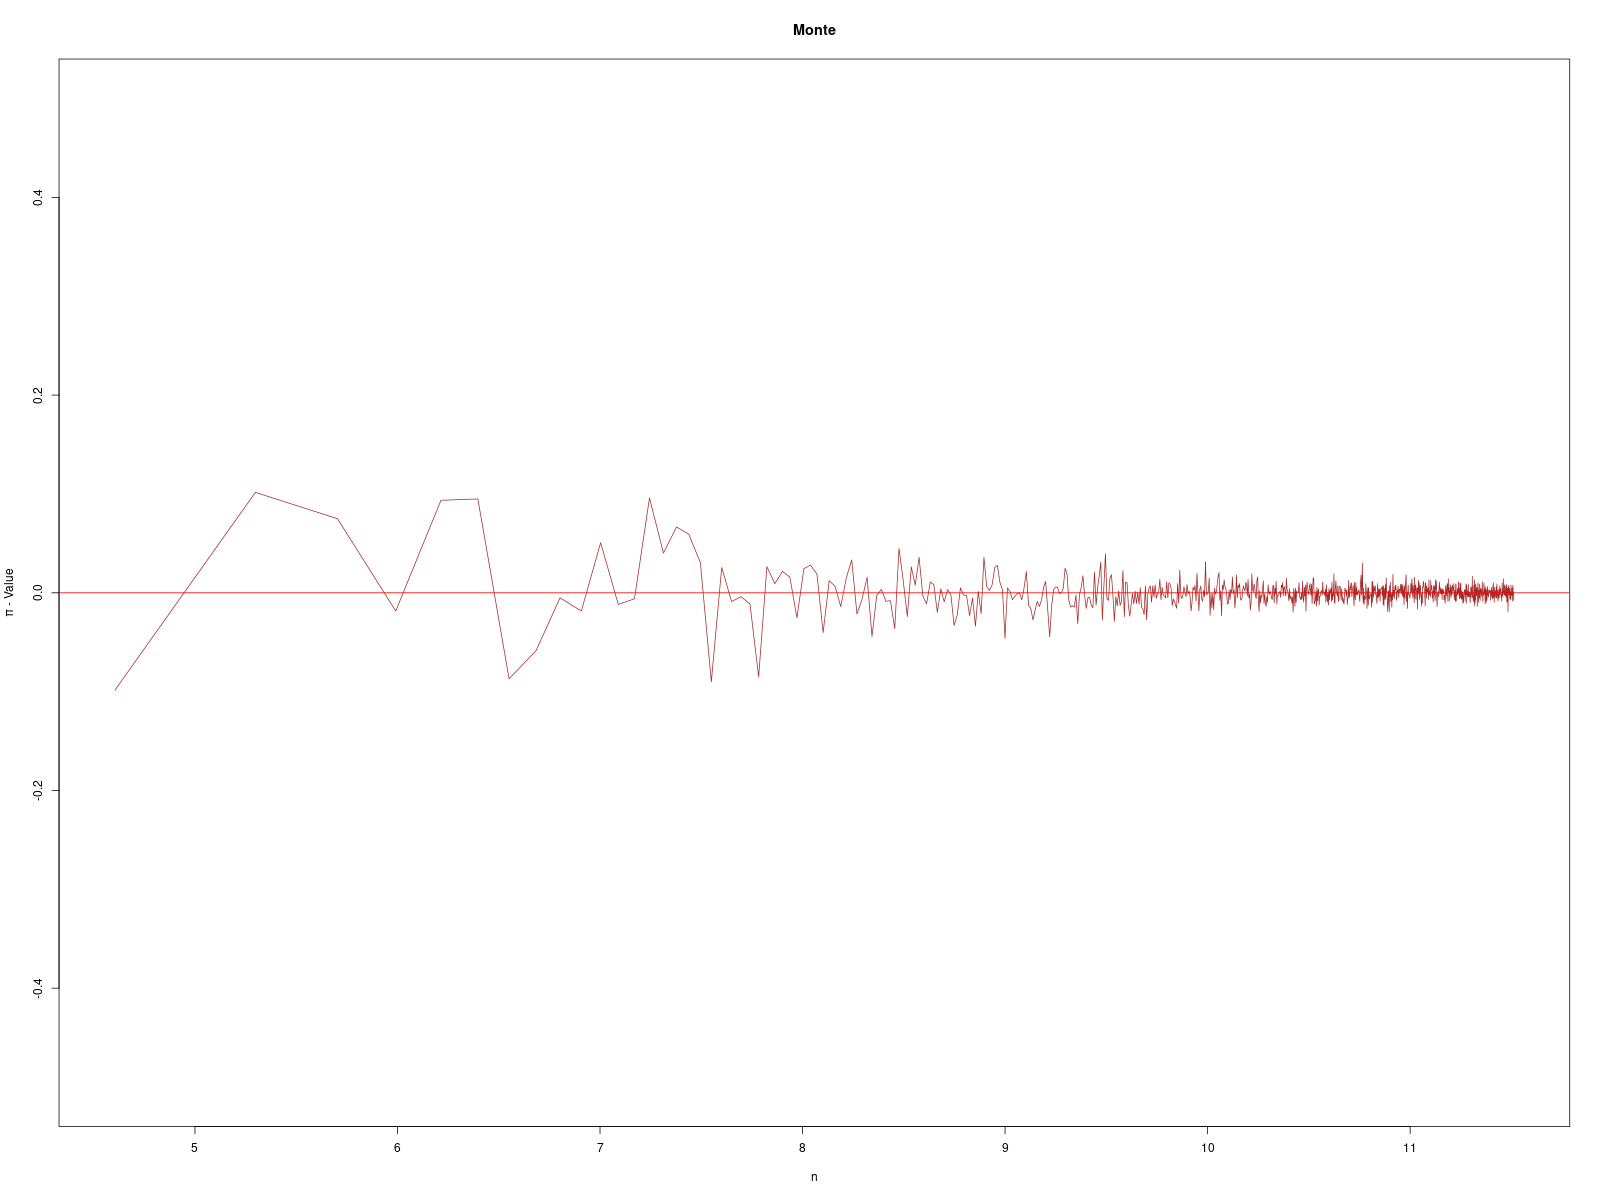
\includegraphics[width=1\textwidth]{~/AlgoNumeryczne/Zadanie1/Grafy/monte_plot.png}
    \caption{Wykres prob.}
    \label{fig:h4}
\end{figure}


\section{wektor vs monte carlo}

\text Metoda monte carlo jest mniej efektywna od metody sumowaniu wektorow, monte carlo jest odpowiednia dla duzego "n" gdzie zlozonosc obliczeniowa sumowania wektorow zaczyna byc coraz wieksza.

\end{document}
